

\documentclass[a4paper]{article}

\usepackage{amsmath}
\usepackage{hyperref}
\usepackage{biblatex}
\usepackage{enumerate}
\usepackage{graphicx}
\usepackage{stmaryrd}
\usepackage[dvipsnames]{xcolor}
\usepackage{listings}
\usepackage{caption}
\usepackage{subcaption}
\usepackage{booktabs}


\addbibresource{refs.bib}

\begin{document}

\author{Ola Bratt \\
  \href{mailto:ola.bratt@gmail.com}{ola.bratt@gmail.com}
  \and
  Patrick Attimont \\
  \href{patrickattimont@gmail.com}{patrickattimont@gmail.com}
}

\title{DAT565/DIT407 Assignment 2}
\date{2024-01-xx}

\maketitle

This paper is addressing the assignment 2 study queries within the \emph{Introduction to Data Science \& AI} course, DIT407 at 
the University of Gothenburg and DAT565 at Chalmers. The main source of information for this project
is derived from the lectures and Skiena~\cite{Skiena:2024}. 
\section*{Problem 1: Scrapping house prices}
Problem 1 have been solved using BeautifulSoup together with simple string operations such as 
\begin{verbatim}
  split, replace and strip, 
\end{verbatim}
also regaular expressions have been used to idefity certain information. The code can be found in the appendix.

\section*{Problem 2: Analyzing 2022 house sales}
To caluculate the five-number summary of the closing prices of the houses prices we simply used 
\begin{verbatim}
describe()
\end{verbatim}
on the dataframe containing the closing prices. The result can be seen in table~\ref{tabular:five_number_summary}.\\

When plotting the histogram of the closing prices, see figure~\ref{fig:histogram_closing_price} we used \emph{square root method} to decide bin size. 
It seems appropriate since it revelas trends without hiding the details. The plot is skewed to the right, which is expected since there are few houses with high prices. 
The plot of closing price vs house area is shown in figure~\ref{fig:closing_price_house_ares}. 
The plot of closing price vs house area with color is shown in figure~\ref{fig:closing_price_house_ares_color}.


\begin{table}
  \begin{center}
  \begin{tabular}{c c}
    min & 250000 \\
    \text{25\%} & 3200000 \\
    \text{50\%} & 4100000 \\
    \text{75\%} & 5035000 \\
    max & 21000000 \\
  \end{tabular}
\end{center}
\caption{Five-number summary of closing prices}
  \label{tabular:five_number_summary}
\end{table}

\newpage

\begin{figure}
  \centering
  \begin{subfigure}[a]{\textwidth}
      \centering
      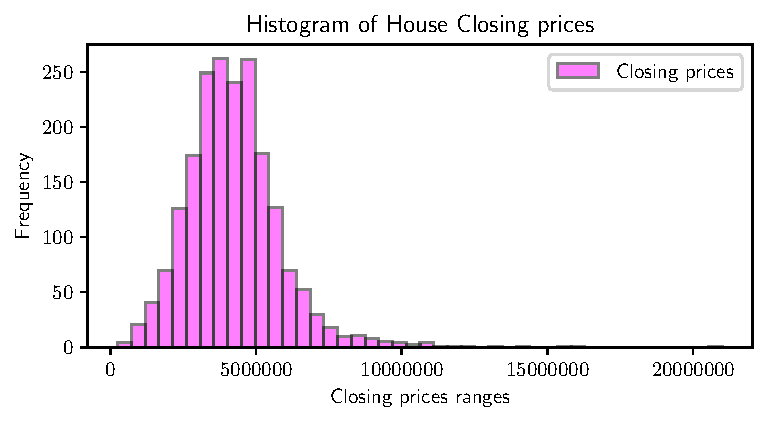
\includegraphics[width=\textwidth]{histogram_closing_price.pdf}
      \caption{Closing prices of houses}
      \label{fig:histogram_closing_price}
  \end{subfigure}
  \vfill
  \begin{subfigure}[b]{\textwidth}
      \centering
      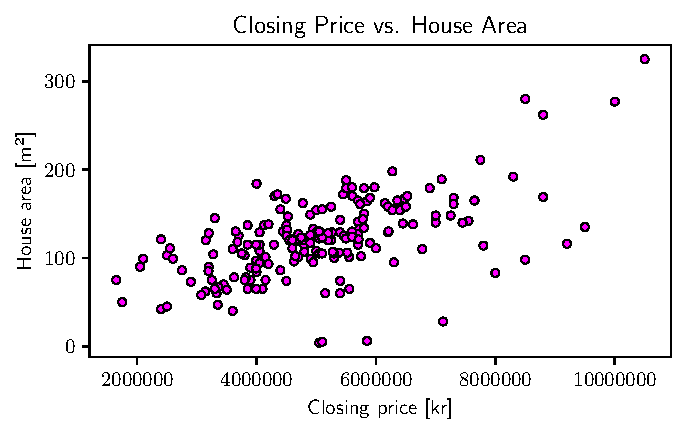
\includegraphics[width=\textwidth]{closing_price_house_ares.pdf}
      \caption{Closing price vs house area}
      \label{fig:closing_price_house_ares}
  \end{subfigure}
  \vfill
  \begin{subfigure}[c]{\textwidth}
      \centering
      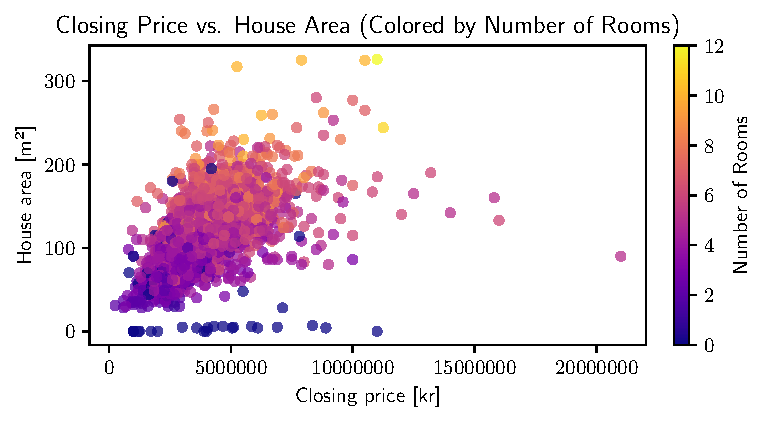
\includegraphics[width=\textwidth]{closing_price_house_ares_color.pdf}
      \caption{Closing price vs house area with color}
      \label{fig:closing_price_house_ares_color}
  \end{subfigure}
     \caption{Plots of house prices}
     \label{fig:house_plots}
\end{figure}


\newpage

\section*{Discussion}

\newpage


\printbibliography

\section*{Appendix: Source Code}

\lstset{
  language=Python,
  basicstyle=\ttfamily,
  commentstyle=\color{OliveGreen},
  keywordstyle=\bfseries\color{Magenta},
  stringstyle=\color{YellowOrange},
  numbers=left,
  basicstyle=\footnotesize,
  breaklines=true,
  postbreak=\mbox{\textcolor{red}{$\hookrightarrow$}\space}
}


\lstinputlisting{ola/assignment2.py}

\end{document}
